\documentclass[11pt]{article}
\usepackage[scaled=0.92]{helvet}
\usepackage{geometry}
\geometry{letterpaper,tmargin=1in,bmargin=1in,lmargin=1in,rmargin=1in}
\usepackage[parfill]{parskip} % Activate to begin paragraphs with an empty line rather than an indent %\usepackage{graphicx}
\usepackage{amsmath,amssymb, mathrsfs, dsfont}
\usepackage{tabularx}
\usepackage[font=footnotesize,labelfont=bf]{caption}
\usepackage{graphicx}
\usepackage{xcolor}
%\usepackage[linkbordercolor ={1 1 1} ]{hyperref}
%\usepackage[sf]{titlesec}
\usepackage{natbib}
\usepackage{../../Tianpei_Report}


\begin{document}
\title{Self-study: Information Metrics and Statistical Divergences}
\author{Tianpei Xie}
\date{ Aug. 19th., 2022 }
\maketitle
\tableofcontents
\newpage
\section{Statistical Divergence}
\subsection{Definitions}
\begin{itemize}
\item \begin{definition}
Given a \emph{differentiable manifold} $\cM$ of dimension $n$, a \underline{\emph{\textbf{divergence}}} on $\cM$ is a $C^{2}$-function $\mathds{D}: \cM\times \cM \to [0,\infty )$  satisfying:
\begin{enumerate}
\item (\textbf{\emph{non-negativity}}) $\divg{}{p}{q} \geq 0$ for all $p,q\in \cM$;
\item (\textbf{\emph{positivity}}) $\divg{}{p}{q} =0$ if and only if $p=q$;
\item At every point $p\in \cM$,  $\divg{}{p}{p+dp}$  is a \emph{\textbf{positive-definite}} quadratic form for infinitesimal displacements $dp$ from $p$. 
\end{enumerate} The last property means that divergence defines an \emph{inner product} on the \emph{\textbf{tangent space}} $T_{p}\cM$ for every $p\in \cM$. Since $\mathds{D}$ is $C^{2}$ on $\cM$, this defines a \emph{\textbf{Riemannian metric}} $g$ on $\cM$.
\end{definition}




\item \begin{definition}
Let $p$, $q$ be $\bR^d \supset \cM_{0}: \rightarrow  \bR$ density functions and let $\alpha \in \bR \setminus \set{1}$. The \emph{\textbf{R\'enyi divergence}} of order $\alpha$ or \underline{\textbf{$\alpha-$divergence}} of a distribution $p$ from a distribution $q$ is defined to be 
\begin{align}
\divg{\alpha}{p}{q} &= \frac{1}{\alpha -1}\log\paren{\E{Q}{\paren{\frac{dP}{dQ}}^{\alpha}}}  = \frac{1}{\alpha -1}\log\paren{\int_{ \cM_{0}}p^{\alpha}(x)q^{1-\alpha}(x)\;  \mu(dx)} \label{eqn: alpha_divg}
\end{align} 
\end{definition}

\item   \begin{definition}
Let $P$ and $Q$ be two probability distributions over a space $\Omega$, such that  $P\ll Q$, that is, $P$ is \emph{\textbf{absolutely continuous}} with respect to $Q$. Then, for a \underline{\emph{\textbf{convex function}}}  $f: [0, +\infty)\to (-\infty ,+\infty]$ such that $f(x)$ is finite for all $x>0$, \underline{$f(1)=0$}, and  \underline{$f(0)=\lim _{t\to 0^{+}}f(t)$} (which could be infinite), the \underline{\emph{\textbf{f-divergence}}} of $P$ from $Q$ is defined as
\begin{align}
\divg{f}{P}{Q} &= \E{Q}{f\paren{\frac{dP}{dQ}}} =  \int_{\Omega} f\paren{\frac{dP}{dQ}} dQ  =  \int_{\Omega} q(x) f\paren{\frac{p(x)}{q(x)}} \mu(dx)  \label{eqn: f_divg}
\end{align} The convex function $f$ is referred as \emph{\textbf{generator function}}.
\end{definition}

\item \begin{definition}
Let $F: \cX \rightarrow \bR$ be a \emph{continuously-differentiable}, \emph{\textbf{strictly convex}} function defined on a convex set $\cX$. The \underline{\textbf{\emph{Bregman divergence}}} associated with $F$ for points $p,q \in \cX$ is the difference between the value of $F$ at point $p$ and the value of the \emph{first-order Taylor expansion} of F around point $q$ evaluated at point $p$:
\begin{align}
\divg{F}{p}{q} &= F(p) - F(q) - \inn{\grad{}{F}(q)}{p - q} \label{eqn: bregman_divg}
\end{align}
\end{definition}

\item \begin{definition}
We suppose $\cX = \cY$ and that for some $p \ge 1$, $c(x,y)= d(x,y)^p$, where $d$ is a distance on $\cX$,  the \underline{\textbf{$p$-Wasserstein distance}} between measures $\alpha, \beta$ on $\cX$ is $\cW_{p}(\alpha, \beta)$, where
\begin{align}
\paren{\cW_{p}(\alpha, \beta)}^{p}:= \min_{\substack{(X, Y) \sim \pi; \\ X_{\#}\pi = \alpha,\\ Y_{\#}\pi = \beta}}& \E{(X,Y)}{d(X, Y)^{p}}\label{eqn: wasserstein_dist}
\end{align}
\end{definition}
\end{itemize}

\subsection{KL Divergence for Exponential Families}
\begin{itemize}
\item The canonical representation of \underline{\emph{\textbf{exponential famlity}}} of distribution has the following form
\begin{align}
p(x_1, \ldots, x_{m}) = p(\mb{x}; \mb{\eta}) &= \exp\paren{\inn{\mb{\eta}}{\mb{\phi}(\mb{x})} - A(\mb{\eta})}h(\mb{x})\nu(d\mb{x}) \nonumber \\
&= \exp\paren{\sum_{\alpha}\eta_{\alpha}\phi_{\alpha}(\mb{x}) -  A(\mb{\eta})} \label{eqn: exp_fam}
\end{align} where $\phi$ is a feature map  and $\mb{\phi}(\mb{x})$ defines a set of \emph{\textbf{sufficient statistics}} (or \emph{\textbf{potential functions}}). The normalization factor is defined as
\begin{align*}
 A(\mb{\eta}) &:= \log \int \exp\paren{ \inn{\mb{\eta}}{\mb{\phi}(\mb{x})} }h(\mb{x})\nu(d\mb{x}) = \log Z(\mb{\eta})
\end{align*} $A(\mb{\eta})$ is also referred as \textbf{\emph{log-partition function}} or \emph{cumulant function}. The parameters $\mb{\eta} = (\eta_{\alpha})$ are called \textbf{\emph{natural parameters}}  or \emph{canonical parameters}. The canonical parameter $\set{\eta_{\alpha}}$ forms a \textbf{natural (canonical) parameter space}
\begin{align}
\Omega = \set{\mb{\eta} \in \bR^{d}: A(\mb{\eta}) < \infty} \label{eqn: canonical_space}
\end{align}

\item The exponential family is the unique solution of \textbf{\emph{maximum entropy estimation}} problem:
\begin{align}
\min_{q \in \Delta}&\quad \kl{q}{p_{0}} \label{eqn: max_ent}\\
\text{s.t.}&\quad \E{q}{\phi_{\alpha}(X)} = \mu_{\alpha}\,\quad  \forall\, \alpha \in \cI   \label{eqn: max_ent_mean_constraint}
\end{align} where $\kl{q}{p_0} = \int \log(\frac{q}{p_0}) q dx = \E{q}{\log\frac{q}{p_0}}$ is the relative entropy or the Kullback-Leibler divergence of $q$ w.r.t. $p_0$.

Here $\mb{\mu} = (\mu_{\alpha})_{\alpha \in \cI}$ is a set of  \textbf{\emph{mean parameters}}. The space of mean parameters $\cM$ is a \emph{convex polytope} spanned by potential functions $\set{\phi_{\alpha}}$.
\begin{align}
\cM &:= \set{\mb{\mu} \in \bR^d: \exists q\,\; \text{s.t. } \E{q}{\phi_{\alpha}(X)} = \mu_{\alpha}\,\quad  \forall\, \alpha \in \cI} = \text{conv}\set{\phi_{\alpha}(x),\; x\in \cX, \;\alpha \in \cI}  \label{eqn: marginal_polytope}
\end{align}

\item Moreover $A(\mb{\eta})$ has a variational form 
\begin{align}
A(\mb{\eta}) &=  \sup_{\mb{\mu} \in \cM}\set{ \inn{\mb{\eta}}{\mb{\mu}} - A^{*}(\mb{\mu})} \label{eqn: log_partition_variational_form}
\end{align}
where $A^{*}(\mb{\mu})$ is the conjugate dual function of $A$ and it is defined as
\begin{align}
A^{*}(\mb{\mu}) &:= \sup_{\mb{\eta} \in \Omega} \set{\inn{\mb{\mu}}{\mb{\eta}} - A(\mb{\eta})} \label{eqn: conjugate_dual_partition}
\end{align}

It is shown that $A^{*}(\mb{\mu})  = -H(q_{\mb{\eta}(\mb{\mu})})$ for $\mb{\mu} \in  \cM^{\circ}$ which is the negative entropy. $A^{*}(\mb{\mu})$ is also the optimal value for the \textbf{maximum likelihood estimation} problem on $p$. The exponential family can be reparameterized according to its mean parameters $\mb{\mu}$ via backward mapping $(\grad{}{A})^{-1}: \cM^{\circ} \rightarrow  \Omega$, called \textbf{mean parameterization}.

\item We can formulate the \textbf{KL divergence} between two distributions in exponential family $\Omega$ using its primal and dual form
\begin{itemize}
\item \textbf{Primal-form}: given $\mb{\eta}_1, \mb{\eta}_2 \in \Omega$
\begin{align}
\kl{p_{\mb{\eta}_1}}{p_{\mb{\eta}_2}} \equiv  \kl{\mb{\eta}_1}{\mb{\eta}_2}
&=  A(\mb{\eta}_2) - A(\mb{\eta}_1) -  \inn{\mb{\mu}_{1}}{\mb{\eta}_2 - \mb{\eta}_1}  \label{eqn: kl_primal}\\
&\equiv  A(\mb{\eta}_2) - A(\mb{\eta}_1) -  \inn{\grad{}{A}(\mb{\eta}_1)}{\mb{\eta}_2 - \mb{\eta}_1}  \nonumber
\end{align}

\item \textbf{Primal-dual form}: given $\mb{\mu}_1 \in \cM, \mb{\eta}_2 \in \Omega$
\begin{align}
 \kl{\mb{\mu}_1}{\mb{\eta}_2} &= A(\mb{\eta}_2) + A^{*}(\mb{\mu}_1) - \inn{\mb{\mu}_{1}}{\mb{\eta}_2}  \label{eqn: kl_primal_dual}
\end{align}

\item \textbf{Dual-form}: given $\mb{\mu}_1, \mb{\mu}_2  \in \cM$
\begin{align}
 \kl{\mb{\mu}_1}{\mb{\mu}_2} &= A^{*}(\mb{\mu}_1) - A^{*}(\mb{\mu}_{2}) - \inn{\mb{\eta}_2}{\mb{\mu}_{1} - \mb{\mu}_{2}}  \label{eqn: kl_dual} \\
 &\equiv  A^{*}(\mb{\mu}_1) - A^{*}(\mb{\mu}_{2}) - \inn{\grad{}{A^{*}}(\mb{\mu}_{2})}{\mb{\mu}_{1} - \mb{\mu}_{2}} \nonumber
\end{align}
\end{itemize}

\item The dual form is related to the \emph{Bregman divergence}, which induce the \textbf{projection operation}.  We see that dual form $\kl{\mb{\mu}_1}{\mb{\mu}_2} = \divg{A^{*}}{\mb{\mu}_1}{\mb{\mu}_2}$, where $F = A^{*}$ is the negative entropy.
\end{itemize}

\subsection{$\alpha$-Divergence Properties}
See papers in \citep{hero2001alpha, nielsen2011r, poczos2011estimation}.
\begin{itemize}
\item $\divg{\alpha}{p}{q} = \divg{1-\alpha}{q}{p}$
\item $\frac{\alpha}{1 - \alpha}\divg{1-\alpha}{p}{q} = \divg{\alpha}{q}{p}$
\item If $\alpha = -1$, $\divg{(-1)}{p}{q} =\divg{(1)}{q}{p} = \kl{p}{q} \equiv \int_{x} p(x)\log\frac{p(x)}{q(x)} dx $ is the \textbf{Kullback-Leibler divergence}. 
\item For $p_{\mb{\eta}_1}, q_{\mb{\eta}_2}$ exponential families, $\alpha$-divergence has closed form expression:
\begin{align}
\divg{\alpha}{p_{\mb{\eta}_1}}{q_{\mb{\eta}_2}} &= \frac{1}{1- \alpha}\paren{\alpha A(\mb{\eta}_1) + (1-\alpha) A(\mb{\eta}_2) - A(\alpha \mb{\eta}_1 + (1- \alpha)\mb{\eta}_2)} \label{eqn: alpha_divg_exp_fam}
\end{align} where $A(\mb{\eta})$ is the \textbf{\emph{log-partition function}} or \emph{cumulant function}.
\end{itemize}

\subsection{$f$-Divergence Properties}
For more details see tutorials in \citep{csiszar2004information, liese2006divergences} and see lecture notes in \citep{polyanskiy2014lecture}.
\begin{itemize}
\item $\divg{f_1 + f_2}{p}{q} = \divg{f_1}{p}{q} + \divg{f_2}{p}{q}$

\item $\divg{f}{p}{q} = \divg{g}{p}{q}$ if $f(x) = g(x) + c(x-1)$ for some $c\in \bR$

\item \emph{\textbf{Reversal by convex inversion}}: for any function $f$, its \emph{\textbf{convex inversion}} is defined as $g(t):=tf(1/t)$. If $f$ satisfies condition for $f$-divergence, then $g$ satisfies the condition as well and $\divg{g}{Q}{P} = \divg{f}{P}{Q}$.

\item \emph{\textbf{Data processing inequality}}: if $\kappa$ is an arbitrary transition probability that transforms measures $P$ and $Q$ into $P_{\kappa}$ and $Q_{\kappa}$ correspondingly, then
\begin{align}
\divg{f}{P}{Q} \geq \divg{f}{P_{\kappa }}{Q_{\kappa }}. \label{eqn: f_divg_data_processing_ineq}
\end{align} The equality here holds if and only if the transition is induced from a \emph{\textbf{sufficient statistic}} with respect to $\{P, Q\}$.

\item \textbf{\emph{Joint Convexity}}: for any $0 \le \lambda \le 1$, 
\begin{align}
\divg{f}{\lambda P_{1}+(1-\lambda )P_{2}}{\lambda Q_{1}+(1-\lambda )Q_{2}}  \leq \lambda\divg{f}{P_{1}}{Q_{1}}+ (1-\lambda) \divg{f}{(P_{2}}{Q_{2}}. \label{eqn: f_divg_convex}
\end{align} This follows from the convexity of the mapping $(p,q) \mapsto q\,f(p/q)$  on $\bR _{+}^{2}$.

\item  
\begin{theorem} (\textbf{Variational representations}) \citep{polyanskiy2014lecture, wan2020f}\\
Let $f^{*}$ be the \emph{\textbf{convex conjugate}} of $f$. Let $\mathrm{effdom} (f^{*})$ be the \textit{effective domain} of $f^{*}$, that is,  $\mathrm {effdom} (f^{*})=\{y:\, f^{*}(y)<\infty \}$. Then we have \emph{two \textbf{variational representations}} of $\divg{f}{p}{q}$:
\begin{align}
\divg{f}{P}{Q} &= \sup _{g:\, \Omega\, \to \,\mathrm{effdom} (f^{*})} \E{P}{g} - \E{Q}{f^{*}\circ g} \label{eqn: f_divg_variational_representation}
\end{align}
\end{theorem}

\item Special cases:
\begin{enumerate}
\item \textbf{\emph{KL divergence}} if $f(x) = x \log(x)$:
\begin{align*}
\divg{f}{P}{Q} &= \int_{\Omega}dQ \frac{dP}{dQ} \log\paren{\frac{dP}{dQ}}  = \int_{\Omega} dP  \log\paren{\frac{dP}{dQ}} = \E{P}{\log\paren{\frac{dP}{dQ}} }=  \kl{P}{Q}
\end{align*}

\item \underline{\emph{\textbf{Total Variation divergence}}} if $ f(x)=\frac {1}{2}|x-1|$:
\begin{align}
\divg{f}{P}{Q} &= \frac{1}{2} \E{Q}{\abs{\paren{\frac{dP}{dQ}} - 1}} = \frac{1}{2} \int \abs{dP - dQ} := TV(P\!\parallel \!Q)   \label{eqn: f_divg_tv_divg}
\end{align} It has \emph{variational representation}
\begin{align}
TV(P\!\parallel \!Q) &= \sup_{f \in \text{Lip}_1}\E{P}{f(X)} - \E{Q}{f(X)} = \cW_{1}(P, Q) \label{eqn: f_divg_tv_divg_var}
\end{align} where $\text{Lip}_1 := \set{f : \cX \rightarrow \bR: \norm{f}{\infty} \le 1}$ is Lipschitz function. It is also equal to the Wasserstein-$1$ distance.

\item \underline{\emph{\textbf{$\chi^2$-divergence}}} if $f(x) = (x - 1)^2$:
\begin{align}
\divg{f}{P}{Q} &= \E{Q}{\paren{\frac{dP}{dQ} - 1}^2} = \int_{\Omega} \frac{\paren{dP - dQ}^2}{dQ}  :=\chi^2(P\!\parallel \!Q)  \label{eqn: f_divg_chi2_divg}
\end{align}

\item \underline{\emph{\textbf{Squared Hellinger distance}}}: $f(x) = (1 - \sqrt{x})^2$
\begin{align}
\divg{f}{P}{Q} &= \E{Q}{\paren{1 - \sqrt{\frac{dP}{dQ}}}^2} \nonumber\\
&= \int_{\Omega} \paren{\sqrt{dP} - \sqrt{dQ}}^2 = 2- 2 \int \sqrt{dP\,dQ} := H^2(P\!\parallel \!Q)   \label{eqn: f_divg_hellinger_divg}
\end{align}

\item \underline{\emph{\textbf{Jensen-Shannon divergence}}}: $f(x) = x \log(\frac{2 x}{x + 1}) + \log(\frac{2}{x + 1})$ ,
\begin{align}
\divg{f}{P}{Q} &= \kl{P}{\frac{P + Q}{2}} + \kl{Q}{\frac{P + Q}{2}}  := \divg{JS}{P}{Q}   \label{eqn: f_divg_jensen_divg}
\end{align}

\item  \underline{\emph{\textbf{Hellinger $\alpha$-divergence}}} $\divg{f_{\alpha}}{p}{q}$ is defined by generator 
%\begin{align*}
%f_{\alpha}(x) &:= \left\{ 
%\begin{array}{cc}
%\frac{x^{\alpha} - \alpha x - \left( 1 - \alpha \right)}{\alpha  \left(\alpha - 1 \right)} & \text{if}\ \alpha\neq 0,\, \alpha\neq 1, \\
%    x\log(x)-x+1, & \text{if}\ \alpha=1, \\
%    - \log(x) +x-1, & \text{if}\ \alpha=0
%\end{array}
%\right..
%\end{align*}
\begin{align*}
f^{(\alpha)}(x) &:= \left\{ 
\begin{array}{cc}
\frac{4}{(1-\alpha^2)} \set{1 - x^{\frac{(1+\alpha)}{2}}}& \text{if}\ \alpha\neq \pm 1, \\
    x\log(x), & \text{if}\ \alpha=1, \\
    - \log(x), & \text{if}\ \alpha=-1
\end{array}
\right..
\end{align*} For $\alpha = \pm 1$, it is the KL divergence. For $\alpha \neq \pm 1$, the corresponding divergence is 
\begin{align}
\divg{f^{(\alpha)}}{p}{q} &=\frac{4}{(1-\alpha^2)}\set{1 - \int_{\cX}(p(x))^{\frac{1 + \alpha}{2}}  (q(x))^{\frac{1 - \alpha}{2}} dx } \label{eqn: hellinger_alpha_divergence}
\end{align}

The R\'enyi divergence and Hellinger $\alpha$-divergence has one-to-one correspondence
\begin{align*}
\divg{\frac{\alpha + 1}{2}}{p}{q} &= \frac{2}{\alpha - 1}\log\paren{1- \paren{\frac{1 - \alpha^2}{4}}\divg{f^{(\alpha)}}{P}{Q}}.
\end{align*} Note that R\'enyi divergence itself is \textbf{not $f$-divergence}.

We can formulate the \emph{\textbf{dual}} of Hellinger $\alpha$-divergence using \emph{\textbf{the conjugate dual}} of  $(f^{(\alpha)})^{*} = f^{(-\alpha)}$.  When $\alpha = 1$, it is the KL divergence.


\item  \underline{\emph{\textbf{Bregman divergence}}}:
The only $f$-divergence that is also a Bregman divergences is the \textbf{KL divergence}. 
\end{enumerate}


\item $f$-divergence is a \textbf{generalization} of  KL divergence from \emph{\textbf{information theorectial perspective}} \citep{thomas2006elements}. Bregman divergence is a generalization of KL divergence from the \emph{\textbf{projection perspective}} as well as \emph{Generalized Pythagorean Theorem}.
\end{itemize}

\section{Divergence on Statistical Manifolds}
\subsection{Dual Connections}
\begin{itemize}
\item
\begin{definition} 
Let $(S, g)$ be a Riemannian manifold and $\nabla$ and $\nabla^{*}$ are two connections on $TS$. If for all vector fields $X, Y, Z \in \frX(S)$, 
\begin{align}
Z\inn{X}{Y} &= \inn{\nabla_{Z}{X}}{Y} + \inn{X}{\nabla^{*}_{Z}(Y)}   \label{eqn: dual_connections}
\end{align} holds, then we say that $\nabla$ and $\nabla^{*}$ are \emph{\textbf{duals}} to each other with respect to the Riemannian metric $g$. We call one either \underline{\emph{\textbf{the dual connection}}}   or \underline{\emph{\textbf{the conjugate connection}}}.

We call the triple $(g, \nabla, \nabla^{*})$ \underline{\emph{\textbf{a dualistic structure}}} on $S$.
\end{definition}

\item We see that the coefficients $\Gamma_{i,j;k}$ and $\Gamma^{*}_{i,j;k}$ for $\nabla$ and $\nabla^{*}$ have the relationship:
\begin{align*}
\partial_k\,g_{i,j} &= \Gamma_{k,i; j} + \Gamma_{k,j; i}^{*}
\end{align*}

\item Similarly, define \emph{\textbf{the covariant derivative}} of vector field \emph{along curve} with respect to $\nabla$ and its dual connection $\nabla^{*}$ as $D_t$ and $D_t^{*}$, then 
\begin{align*}
\frac{d}{dt}\inn{X(t)}{Y(t)} &= \inn{D_tX(t)}{Y(t)} + \inn{X(t)}{D_t^{*}Y(t)}
\end{align*}

\item For \emph{\textbf{the parallel transport map}} $\Pi_{\gamma}$ and $\Pi^{*}_{\gamma}$ along the curve $\gamma$ (from $t_0$ to $t_1$) with respect to $\nabla$ and its dual $\nabla^{*}$, we have 
\begin{align*}
\inn{\Pi_{\gamma}(X)}{\Pi^{*}_{\gamma}(Y)}_q &= \inn{X}{Y}_p.
\end{align*} where $p=\gamma(t_0)$ and $q = \gamma(t_1)$. This is a generalization of ``\emph{\textbf{the \underline{invariance} of the inner product under \underline{parallel translation} with respect to \underline{metric connections}}}."

\item Also \emph{\textbf{the Riemannian curvature tensor}} with respect to $\nabla$ and its dual $\nabla^{*}$ has the relationship
\begin{align*}
\inn{R(X,Y)Z}{W} &= -\inn{R^{*}(X,Y)Z}{W}.
\end{align*} Thus $Rm = -Rm^{*}$, so $R = 0 \Leftrightarrow R^{*} = 0$. 

In other word, \emph{a Riemannian manifold $S$ with dualistic structure $(g, \nabla, \nabla^{*})$ is \underline{\textbf{flat} in $\nabla$} \textbf{if and only} if it is \underline{\textbf{flat} in its \textbf{dual connection} $\nabla^{*}$}}.


\item It is clear that if $\nabla$ is \emph{\textbf{a metric connection}}, then $\nabla = \nabla^{*}$. The concept of dual connections $(\nabla, \nabla^{*})$ is a generalization of the metric connection. Moreover, $\frac{1}{2}(\nabla + \nabla^{*})$ becomes \emph{a metric connection}. 


\item Within $\alpha$-connections, $(\nabla^{(-\alpha)}, \nabla^{(\alpha)})$ are \textbf{\emph{duals}} to each other with respect to \emph{the Fisher metric}. Specifically, $(\nabla^{(m)}, \nabla^{(e)})$, i.e. \textit{\textbf{the mixture connection} and \textbf{the exponential connection} are \textbf{duals} to each other}.

From above statement, we see that 
\begin{align}
S \text{ is $(\alpha)$-flat } \Leftrightarrow S \text{ is $(-\alpha)$-flat }\label{eqn: dual_flat}
\end{align} That $(S, g, \nabla, \nabla^{*})$ is called \underline{\emph{\textbf{a dually flat space}}}

\item \begin{remark}
\emph{The exponential family} is \emph{a dually flat space} since it is both \emph{\textbf{$1$-flat}} and \textbf{$(-1)$-flat}. The former corresponds to \underline{\emph{\textbf{the natural parameterization}}} $(\xi^i)$ which is \emph{\textbf{$\nabla^{(e)}$-affine}} and the latter corresponds to \underline{\emph{\textbf{the mean parameterization}}} $(\mu_i)$ which is \emph{\textbf{$\nabla^{(m)}$-affine}}.  It has \emph{\textbf{two mutually dual coordinate systems}}.
\end{remark}
\end{itemize}
\subsection{Divergence as General Contrast Function}
\begin{itemize}
\item \begin{definition}
Let $S$ be a statistical manifold. $D$ is a smooth function $D = \divg{}{\cdot}{\cdot}: S \times S  \rightarrow  \bR$ satisfying for any $p,q \in S$
\begin{align}
\divg{}{p}{q} > 0,  \text{ and }  \divg{}{p}{q} = 0, \; \text{ iff }p=q.
  \label{eqn: divergence_def}
\end{align}
\end{definition}

\item The divergence function usually does not define a \emph{distance function} since it does not satisfy the \emph{\textbf{symmetry}} and \emph{\textbf{triangle inequality}} condition. 

\item Given smooth chart $(U, (\xi^i))$ in $S$, let us represent \emph{\textbf{a pair of points}} $(p, \widetilde{p}) \in S \times S$ by a pair of coordinates $((\xi^i), (\widetilde{\xi}^i))$ and denote \emph{\textbf{the partial derivatives}} of $\divg{}{p}{\widetilde{p}}$ with respect to $p$ and $\widetilde{p}$ by
\begin{align*}
\widehat{\mathds{D}}\left( (\partial_i)_p \;\Bigr\|\;  \widetilde{p} \right) :=\widehat{\mathds{D}}\left( \partdiff{}{\xi^i}\Bigr|_{p} \;\Bigr\|\;  \widetilde{p} \right) &:= \partdiff{}{\xi^i}\Bigr|_{p}\divg{}{p}{\widetilde{p}} \\
\widehat{\mathds{D}}\left( (\partial_i)_p \;\Bigr\|\;  (\widetilde{\partial}_j)_{\widetilde{p}}  \right)  := \widehat{\mathds{D}}\left( \;\partdiff{}{\xi^i}\Bigr|_{p} \;\Bigr\| \; \partdiff{}{\widetilde{\xi}^j}\Bigr|_{\widetilde{p}} \;\right) &:= \partdiff{}{\xi^i}\Bigr|_{p} \partdiff{}{\widetilde{\xi}^j}\Bigr|_{\widetilde{p}}  \divg{}{p}{\widetilde{p}} \\
\widehat{\mathds{D}}\left( (\partial_i\partial_j)_p \;\Bigr\|\;  (\widetilde{\partial}_k)_{\widetilde{p}}  \right) := \widehat{\mathds{D}}\left( \;\partdiff{}{\xi^i}\partdiff{}{\xi^j}\Bigr|_{p} \;\Bigr\| \; \partdiff{}{\widetilde{\xi}^k}\Bigr|_{\widetilde{p}} \;\right) &:= \paren{\partdiff{}{\xi^i}\partdiff{}{\xi^j}}\Bigr|_{p}  \partdiff{}{\widetilde{\xi}^k}\Bigr|_{\widetilde{p}}  \divg{}{p}{\widetilde{p}} \\
\cdots 
\end{align*}
Here with abuse of notations, we consider the function $\widehat{\mathds{D}}(\;\cdot \;\|\; \cdot\;) $ as $T_{p}S \times T_{\widetilde{p}}S \rightarrow \bR$, where the derivation operation on $p$ and $\widetilde{p}$ are separated into two sides. Similarly, we have
\begin{align*}
\widehat{\mathds{D}}\left( \paren{X_1 \xdotx{,} X_l}_{p} \;\Bigr\|\;  \widetilde{p} \right) \quad \text{ and } \quad  \widehat{\mathds{D}}\left( p \;\Bigr\|\;  \paren{Y_1 \xdotx{,} Y_m}_{\widetilde{p}} \right) \\
\text{ and }\widehat{\mathds{D}}\left( \paren{X_1 \xdotx{,} X_l}_{p} \;\Bigr\|\;   \paren{Y_1 \xdotx{,} Y_m}_{\widetilde{p}} \right)
\end{align*} Now we consider \emph{\textbf{their restrictions onto the diagonal}} $\{(p, p) : p \in S\} \subset S \times S $ and denote the functions induced on $S$ by
\begin{align*}
\widehat{\mathds{D}}\left[ X_1 \xdotx{,} X_l \;\Bigr\|\;  \cdot \right]  &: p \mapsto \widehat{\mathds{D}}\left( \paren{X_1 \xdotx{,} X_l}_{p} \;\Bigr\|\;  p \right)\\
\widehat{\mathds{D}}\left[ \cdot \;\Bigr\|\;  Y_1 \xdotx{,} Y_m \right] &:  p \mapsto \widehat{\mathds{D}}\left( p \;\Bigr\|\;  \paren{Y_1 \xdotx{,} Y_m}_{p} \right) \\
\text{ and }\widehat{\mathds{D}}\left[X_1 \xdotx{,} X_l \;\Bigr\|\;   Y_1 \xdotx{,} Y_m \right] &:  p \mapsto \widehat{\mathds{D}}\left( \paren{X_1 \xdotx{,} X_l}_{p} \;\Bigr\|\;   \paren{Y_1 \xdotx{,} Y_m}_{p} \right)
\end{align*}

It follows from the definition that at $p=q$ is the \emph{\textbf{miniminer}} of $\divg{}{p}{q}$ and $\divg{}{q}{p}$ so
\begin{align}
\widehat{\mathds{D}}\left[ \partial_i \;\|\;  \cdot \right] &= \widehat{\mathds{D}}\left[ \cdot  \;\|\; \partial_i  \right] = 0,\quad i=1 \xdotx{,} n \label{eqn: derivation_divergence} 
\end{align}
The \emph{\textbf{Hessian} of function $\mathds{D}$} is defined as 
\begin{align}
\widehat{\mathds{D}}\left[ \partial_i \partial_j \;\|\; \cdot \right] = \partdiff{}{\xi^i}\partdiff{}{\xi^j}\Bigr|_{p=q}\divg{}{p}{q}:= g_{i,j}^{D}(q)  \label{eqn: derivation_divergence_metric} 
\end{align} We can also show that
\begin{align*}
\widehat{\mathds{D}}\left[ \partial_i \partial_j \;\|\; \cdot \right] = \widehat{\mathds{D}}\left[\cdot   \;\|\; \partial_i \partial_j \right] = - \widehat{\mathds{D}}\left[ \partial_i  \;\|\; \partial_j\right] 
\end{align*}


 \item \begin{definition}
Let $S$ be a statistical manifold. a \underline{\emph{\textbf{(statistical) divergence}}} or \emph{\textbf{contrast function}} is a smooth function $\mathds{D} = \divg{}{\cdot}{\cdot}: S \times S  \rightarrow  \bR$ satisfying for any $p,q \in S$
\begin{enumerate}
\item $\divg{}{p}{q} > 0$
\item $\divg{}{p}{q} = 0$ iff $p =q$
\item At each $p=q \in S$, \emph{\textbf{the Hessian matrix}} of $\divg{}{p}{q}$, $[g_{i,j}^{D}]_{p}$ is \emph{\textbf{strictly positive definite}} where
\begin{align*}
g_{i,j}^{(D)} :=  \widehat{\mathds{D}}\left[ \partial_i \partial_j \;\|\; \cdot \right] =  \widehat{\mathds{D}}\left[ \cdot \;\|\; \partial_i \partial_j  \right] = - \widehat{\mathds{D}}\left[  \partial_i  \;\|\;\partial_j  \right] 
\end{align*}
\end{enumerate}
\end{definition}

\item For a divergence $\mathds{D}$, a \underline{\emph{\textbf{unique Riemannian metric}}} $g^{(D)} = \inn{}{}^{(D)}$ on $S$ is defined by $g_{i,j}^{(D)} := \inn{\partial_i}{\partial_j}^{(D)}$, or equivalently by, for $X, Y \in \frX(S)$,
\begin{align}
\inn{X}{Y}^{(D)} &= -\widehat{\mathds{D}}\left[ X \;\|\;  Y \right]  \label{eqn: inner_product_induced_by_divergence} 
\end{align}

\item This metric gives \emph{\textbf{the second order approximation}} of  $\mathds{D}$ as
\begin{align}
\divg{}{p}{q} &= \frac{1}{2}g_{i,j}^{(D)}(q)\Delta\xi^i\,\Delta\xi^j + o(\norm{\Delta \xi}{2}^2)
\end{align} where $\Delta \xi^i := \xi^i(p) - \xi^i(q)$ and $ o(\norm{\Delta \xi}{2}^2)$ is a term vanishing faster than $\norm{\Delta \xi}{2}^2$ as $p$ tends to $q$.




\item Given a \emph{\textbf{divergence}} $\mathds{D}$, we can also define \underline{\emph{\textbf{an affine connection}}} $\nabla^{(D)}$ with coefficients $\Gamma_{i,j; k}^{(D)}$ by
\begin{align}
\Gamma_{i,j; k}^{(D)} := -\widehat{\mathds{D}}\left[ \partial_i\,\partial_j \;\|\;  \partial_k \right], \label{eqn: coefficient_affine_connection_by_divergence}
\end{align}
or equivalently by
\begin{align}
\inn{\nabla^{(D)}_{X}{Y}}{Z}^{(D)} &= - \widehat{\mathds{D}}\left[ XY \;\|\;  Z \right].  \label{eqn: affine_connection_by_divergence_inn}
\end{align}

\item Note that  $\nabla^{(D)}$ is \emph{\textbf{necessarily symmetric}} 
\begin{align*}
\Gamma_{i,j; k}^{(D)}  = \Gamma_{j,i; k}^{(D)}
\end{align*}

\item Combined with the metric $g^{(D)}$, the connection $\nabla^{(D)}$ gives \emph{\textbf{the third order approximation}} of the divergence $\mathds{D}$: where
\begin{align}
\divg{}{p}{q} &= \frac{1}{2}g_{i,j}^{(D)}(q)\Delta\xi^i\,\Delta\xi^j + \frac{1}{6}h_{i,j,k}^{(D)}(q)\Delta\xi^i\,\Delta\xi^j\Delta\xi^k + o(\norm{\Delta \xi}{2}^3) \label{eqn: divergence_3rd_order_approx}
\end{align} where 
\begin{align}
h_{i,j,k}^{(D)} &:=  \widehat{\mathds{D}}\left[ \partial_i \partial_j \partial_k \;\|\; \cdot \right]  \label{eqn: divergence_3rd_order_coefficient}
\end{align}
Indeed, the coefficients $h_{i,j,k}^{(D)}$ are determined from $g^{(D)}$ and $\Gamma_{i,j; k}^{(D)}$ by
\begin{align*}
h_{i,j,k}^{(D)} &= \partial_i\,g_{j,k}^{(D)} + \Gamma_{j,k; i}^{(D)}
\end{align*}




\item Let us replace the \emph{divergence} $\mathds{D}(p \| q)$ with its \underline{\emph{\textbf{dual divergence}} $\mathds{D}^{*}(p \| q) = \mathds{D}(q \| p)$}.
Then we obtain $g^{(D^{*})} =g^{(D)}$ and
\begin{align}
\Gamma_{i,j; k}^{(D^{*})} := -\widehat{\mathds{D}}\left[\partial_k   \;\|\; \partial_i\,\partial_j  \right] \label{eqn: coefficient_affine_connection_by_dual_divergence}
\end{align}
Now it is easy to see the following theorem.

\begin{theorem}
$\nabla^{(D)}$ and $\nabla^{(D^{*})}$ are \textbf{dual} with respect to $g^{(D)}$.
\end{theorem}

\item Moreover, we see that
\begin{align*}
\divg{}{p}{q} = \divg{*}{q}{p} &= \frac{1}{2}g_{i,j}^{(D^{*})}(p)(-\Delta\xi^i)\,(-\Delta\xi^j) + \frac{1}{6}h_{i,j,k}^{(D^{*})}(p)(-\Delta\xi^i)\,(-\Delta\xi^j)(-\Delta\xi^k )+ o(\norm{\Delta \xi}{2}^3) \\
&= \frac{1}{2}g_{i,j}^{(D)}(p)\Delta\xi^i\,\Delta\xi^j - \frac{1}{6}h_{i,j,k}^{(D^{*})}(p)\Delta\xi^i\Delta\xi^j\Delta\xi^k + o(\norm{\Delta \xi}{2}^3)
\end{align*}
Thus
\begin{align*}
h_{i,j,k}^{(D^{*})} &:=  \widehat{\mathds{D}}\left[ \cdot  \;\|\;   \partial_i \partial_j \partial_k\right]  = \partial_i g_{j,k}^{(D)}  + \Gamma_{j,k;i}^{(D^{*})}
\end{align*}

We thus see that \underline{\emph{\textbf{any divergence induces a torsion-free dualistic structure}}}.

\item  \emph{\textbf{Conversely}},  \emph{any triple $(g^{(D)}, \nabla, \nabla^{*})$ of a \textbf{metric} and \textbf{mutually dual symmetric connections} are \textbf{induced from a divergence}}. \citep{amari2007methods}.

\item \begin{remark}
For each \emph{\textbf{divergence}} $\mathds{D}$ and its dual $\mathds{D}^{*}$, we can construct \emph{a \underline{\textbf{dualist structure}} $(g^{(D)}, \nabla^{(D)}, \nabla^{(D^{*})})$ on statistical manifold} $S$, where \emph{\textbf{the Riemannian metric}} $g^{(D)}$ is the \emph{\textbf{Hessian}} of $\mathds{D}$ at $p=q$, and the \emph{\textbf{coefficients}} of connections $\Gamma_{i,j; k}^{(D)}$ and $\Gamma_{i,j; k}^{(D^{*})}$ are computed in \eqref{eqn: coefficient_affine_connection_by_divergence} and \eqref{eqn: coefficient_affine_connection_by_dual_divergence}, respectively.
\end{remark}
\end{itemize}

\subsection{Induced Connections from KL-Divergence and $f$-Divergence}
\begin{itemize}
\item \begin{example}
Consider the KL divergence:
\begin{align*}
\kl{p(x; \xi)}{q(x; \widetilde{\xi})} &= \int_{\cX}p(x; \xi) \log p(x; \xi)  dx - \int_{\cX}p(x; \xi) \log q(x; \widetilde{\xi})  dx  \\
\widehat{\mathds{D}}^{KL}\left[ \partial_i \;\|\;  \cdot \right]  &= (\partial_i)_{p}\paren{\int_{\cX}p(x; \xi) \log p(x; \xi)  dx - \int_{\cX}p(x; \xi) \log q(x; \widetilde{\xi})  dx} \\
&= \int_{\cX} \paren{(\partial_i)_{p} p(x; \xi)} \log p(x; \xi)  dx + \int_{\cX} \paren{(\partial_i)_{p} \log p(x; \xi)} p(x; \xi)   dx \\
& \quad  - \int_{\cX} \paren{(\partial_i)_{p} p(x; \xi)} \log q(x; \widetilde{\xi})  dx \\
&\text{since }\int_{\cX}  (\partial_i \log p) p dx = \int_{\cX} (\partial_i p)\, p^{-1} p dx = \int_{\cX} (\partial_i p)\,  dx  = 0\\
&= \int_{\cX} \paren{(\partial_i)_{p} p(x; \xi)} \log p(x; \xi)  dx -  \int_{\cX} \paren{(\partial_i)_{p} p(x; \xi)} \log q(x; \widetilde{\xi})  dx \\
\widehat{\mathds{D}}^{KL}\left[ \partial_i \;\|\;  \widetilde{\partial_j} \right]  &= ( \widetilde{\partial_j})_p\brac{\int_{\cX} (\partial_i p(x; \xi)) \log p(x; \xi)  dx -  \int_{\cX} (\partial_i p(x; \xi))  \log q(x; \widetilde{\xi})  dx} \\
&= -\int_{\cX} \paren{(\partial_i)_p p(x; \xi)}  \paren{(\widetilde{\partial}_j)_p\log q(x; \widetilde{\xi})}  dx \\
&= -\int_{\cX} \paren{(\partial_i)_p \log p(x; \xi)}  \paren{(\widetilde{\partial}_j)_p\log q(x; \widetilde{\xi})}  p(x; \xi) dx \\
\Rightarrow  g_{i,j}^{KL} = -\widehat{\mathds{D}}^{KL}\left[ \partial_i \;\|\;  \partial_j \right]&=  \int_{\cX} \paren{(\partial_i)_p \log p(x; \xi)}  \paren{({\partial}_j)_p\log p(x; {\xi})}  p(x; \xi) dx = g_{i,j}.
\end{align*}
\end{example}

\item \begin{example}
Consider the $f$-divergence, where $f$ is convex i.e. $f''(x) > 0$ and $f(1) = 0$
\begin{align}
\divg{f}{p(x; \xi)}{q(x; \widetilde{\xi})} &= \int_{\cX}q(x; \widetilde{\xi}) f\paren{\frac{p(x; \xi)}{q(x; \widetilde{\xi})}} dx  \nonumber\\
\widehat{\mathds{D}}^{f}\left[ \partial_i \;\|\;  \cdot \right] &= - \int_{\cX}((\partial_i)_p p(x; \xi))  f'\paren{\frac{p(x; \xi)}{q(x; \widetilde{\xi})}} dx  \nonumber\\
\widehat{\mathds{D}}^{f}\left[ \partial_i \;\|\;  \widetilde{\partial}_j \right]  &= - \int_{\cX}\{(\partial_i)_p p(x; \xi)\}\{(\widetilde{\partial}_j)_p q(x; \widetilde{\xi})\} \paren{\frac{p(x; \xi)}{q^2(x; \widetilde{\xi})}} f''\paren{\frac{p(x; \xi)}{q(x; \widetilde{\xi})}} dx \nonumber\\
&= - \int_{\cX}\{(\partial_i)_p \log p(x; \xi)\}\{(\widetilde{\partial}_j)_p \log q(x; \widetilde{\xi})\} \paren{\frac{p(x; \xi)}{q(x; \widetilde{\xi})}}^2 f''\paren{\frac{p(x; \xi)}{q(x; \widetilde{\xi})}} q(x; \widetilde{\xi}) dx \nonumber\\
&= - \E{q}{\{(\partial_i)_p \log p(x; \xi)\}\{(\widetilde{\partial}_j)_p \log q(x; \widetilde{\xi})\} \paren{\frac{p(x; \xi)}{q(x; \widetilde{\xi})}}^2 f''\paren{\frac{p(x; \xi)}{q(x; \widetilde{\xi})}}} \nonumber\\
\Rightarrow  g_{i,j}^{D^f} = -\widehat{\mathds{D}}^{f}\left[ \partial_i \;\|\;  \partial_j \right] &:=f''(1)   \int_{\cX}\{(\partial_i)_p \log p(x; \xi)\}\,\{({\partial}_j)_p \log p(x; {\xi})\}\;   p(x; {\xi})  dx = f''(1) g_{i,j}  \label{eqn: riemannian_metric_f_divg}
\end{align}
\end{example}


\item \begin{example}
We can check on the connection induced by the KL divergence and $f$-divergence:
\begin{enumerate}
\item For \textbf{KL-divergence}, \emph{the induced Riemannian metric is the \textbf{Fisher metric}} $g_{i,j}$ and \emph{the induced affine connection} induced by  is 
\begin{align}
\Gamma_{i,j;k}^{(KL)} :=- \widehat{\mathds{D}}^{KL}\left[ \partial_i\,\partial_j \;\|\;  {\partial}_k \right] &= \E{p}{\set{\partial_i \partial_j \ell  + (\partial_i \ell)(\partial_j \ell)} (\partial_k \ell)} = \Gamma_{i,j;k}^{(-1)}  \label{eqn: kl_divergence_affine_connection}
\end{align}  It is \underline{\emph{\textbf{the mixture connection}}} $\nabla^{(-1)}=\nabla^{(m)}$ with respect to \emph{the Fisher metric}.

\item For \textbf{$f$-divergence}, \emph{the induced Riemannian metric is the \underline{\textbf{(scaled) Fisher metric}}} with scaling factor $f''(1)$. 
\begin{align*}
 - \widehat{\mathds{D}}^{f}\left[ \partial_i \partial_j \;\|\;  \widetilde{\partial}_k \right] &= \partial_i\int_{\cX}\paren{\frac{p_{\xi}}{q_{\widetilde{\xi}}}}^2 f''\paren{\frac{p_{\xi}}{q_{\widetilde{\xi}}}} \{(\partial_j)_p \log p_{\xi}\}\,\{(\widetilde{\partial}_k)_p \log q_{\widetilde{\xi}}\}\;   q_{\widetilde{\xi}}  dx \\
 &= \int_{\cX}\set{\brac{2\paren{\frac{p_{\xi}}{q_{\widetilde{\xi}}}} f''\paren{\frac{p_{\xi}}{q_{\widetilde{\xi}}}} + \paren{\frac{p_{\xi}}{q_{\widetilde{\xi}}}}^2 f^{(3)}\paren{\frac{p_{\xi}}{q_{\widetilde{\xi}}}}}\paren{\frac{p_{\xi}}{q_{\widetilde{\xi}}}} \{(\partial_i)_p  \log p_{\xi}\}\, } \times \\
 &\quad  \{(\partial_j)_p \log p_{\xi}\}\,\{(\widetilde{\partial}_k)_p \log q_{\widetilde{\xi}}\}\;   q_{\widetilde{\xi}}  dx \\
 &\quad + \int_{\cX}\paren{\frac{p_{\xi}}{q_{\widetilde{\xi}}}}^2 f''\paren{\frac{p_{\xi}}{q_{\widetilde{\xi}}}}  \{(\partial_i \partial_j)_p \log p_{\xi}\}\,\{(\widetilde{\partial}_k)_p \log q_{\widetilde{\xi}}\}\;    q_{\widetilde{\xi}}  dx
\end{align*}
The \emph{\textbf{induced affine connection}} by $f$-divergence is
\begin{align}
\Gamma_{i,j;k}^{(D_f)} &:= - \widehat{\mathds{D}}^{f}\left[ \partial_i \partial_j \;\|\;  \partial_k \right] =\E{p}{\set{f''(1)\partial_i \partial_j \ell + \paren{2f''(1) + f^{(3)}(1)}(\partial_i \ell)(\partial_j \ell)}(\partial_k \ell)} \label{eqn: f_divergence_affine_connection}
\end{align}
\end{enumerate}
\end{example} 


\item  \begin{example} 
As for the \emph{\textbf{dual divergence}} and \emph{\textbf{dual connections}}, we have the following statement: 
\begin{enumerate}
\item For \textbf{KL-divergence}, its \emph{dual} $\mathds{KL}^{*}\left( p \left\|\right. q \right) = \kl{q}{p}$, \emph{\textbf{the affine connection}} induced by $\mathds{KL}^{*}$ is \emph{\textbf{the exponential connection}} $\nabla^{KL^{*}} = \nabla^{(1)} = \nabla^{(e)}$.
\item For \textbf{$f$-divergence}, its dual $\divg{g}{p}{q} = \divg{f}{q}{p}$ where $g(t) = t f(1/t)$ is \emph{\textbf{the convex inversion}} of $f$. Thus the induced connection
\begin{align*}
\Gamma_{i,j;k}^{(D_g)} &:= - \widehat{\mathds{D}}^{g}\left[ \partial_i \partial_j \;\|\;  \partial_k \right] = - \widehat{\mathds{D}}^{f}\left[ \partial_k  \;\|\; \partial_i \partial_j  \right] = \Gamma_{i,j;k}^{(D_f^{*})}
\end{align*} Note that $g'(t) = f(1/t) - (1/t)\,f'(1/t)$, $g''(t) = (1/t)^3\,f''(1/t)$, $g^{(3)}(t) = -3 t^{-4}f''(t^{-1}) - t^{-5}f^{(3)}(t^{-1})$ so $g''(1) = f''(1)$ and $g^{(3)}(1)= -3 f''(1) - f^{(3)}(1)$. So \emph{\textbf{the dual connection}} is
\begin{align*}
\Gamma_{i,j;k}^{(D_f^{*})} &:=\E{p}{\set{f''(1)\partial_i \partial_j \ell - \paren{f''(1) + f^{(3)}(1)}(\partial_i \ell)(\partial_j \ell)}(\partial_k \ell)}  
\end{align*}
\end{enumerate}
\end{example}
\end{itemize}

\subsection{Hellinger $\alpha$-Divergence and $\alpha$-Connection}
\begin{itemize}
\item Now consider the $f$-divergence $\divg{f^{(\beta)}}{p}{q}$ with the following $f$ function:
\begin{align*}
f^{(\beta)}(x) &:= \left\{ 
\begin{array}{cc}
\frac{4}{(1-\beta^2)} \set{1 - x^{\frac{(1+\beta)}{2}}}& \text{if}\ \beta\neq \pm 1, \\
    x\log(x), & \text{if}\ \beta=1, \\
    - \log(x), & \text{if}\ \beta=-1
\end{array}
\right..
\end{align*} This is the \underline{\emph{\textbf{Hellinger $\alpha$-divergence}}} as discussed above. (Note that in \citep{amari2007methods} the definition of $f$-divergence is the dual of the standard $f$-divergence definition. As a result, the Hellinger $\alpha$-divergence is the book is also the dual of the standard one. We need to replace \underline{$\beta = - \alpha$} to recover the book's definition.) For $\beta = 1$, it is the KL divergence and  $\beta = -1$ it is the dual of KL divergence. For $\beta \neq \pm 1$, the corresponding divergence is 
\begin{align*}
\divg{f^{(\beta)}}{p}{q} &=\frac{4}{(1-\beta^2)}\set{1 - \int_{\cX}(p(x))^{\frac{1+ \beta}{2}} (q(x))^{\frac{1 - \beta}{2}}dx } 
\end{align*}
Then for $\beta \neq \pm 1$, $\frac{d}{dt}f^{(\beta)} = - \frac{2}{1 - \beta} x^{\frac{\beta - 1}{2}} $ and  $\frac{d^2}{dt^2}f^{(\beta)} = x^{\frac{\beta - 3}{2}}$ so that $f''(1) = 1$. $\frac{d^3}{dt^3}f^{(\beta)} = \frac{\beta - 3}{2}x^{\frac{\beta - 5}{2}}$ and $f^{(3)}(1) = \frac{\beta - 3}{2}.$

Substitute the formula $f^{(\beta)}(x)$ into the \eqref{eqn: f_divergence_affine_connection}
\begin{align}
\Gamma_{i,j;k}^{(D_f^{(\beta)})} &=\E{p}{\set{f''(1)\partial_i \partial_j \ell + \paren{2f''(1) + f^{(3)}(1)}(\partial_i \ell)(\partial_j \ell)}(\partial_k \ell)} \nonumber\\
&=  \E{p}{\set{\partial_i \partial_j \ell +  \frac{1 + \beta}{2}(\partial_i \ell)(\partial_j \ell)}(\partial_k \ell)}  \label{eqn: hellinger_alpha_divergence_affine_connection}
\end{align}
For $\beta = 1$, we reconstruct the same formula as in \eqref{eqn: kl_divergence_affine_connection}.

\item Recall that  \underline{\emph{\textbf{the $\alpha$-connections}}} \citep{amari2007methods} $\nabla^{(\alpha)}$ as \emph{\textbf{a family of affine connections}} on the tangent bundle $TS$. The \emph{\underline{\textbf{coefficient of the $\alpha$-connection}}} under \emph{\textbf{the Fisher metric}} is formulated as
\begin{align}
\Gamma_{i,j; k}^{(\alpha)} &= \E{p}{\paren{ \partial_i \partial_j \ell + \frac{1 - \alpha}{2} (\partial_i \ell) (\partial_j \ell)}\paren{\partial_k \ell}} \label{eqn: alpha_connection_coefficient} 
\end{align} 

\item \begin{remark}
Thus we show that \emph{\textbf{\underline{the $\alpha$-connection} with respect to the Fisher metric $g$ is the induced affine connection by the \underline{the Hellinger $\alpha$-divergence}}} in  \eqref{eqn: hellinger_alpha_divergence}. And  \emph{\textbf{the induced dualistic structure} $(g^{(D_f^{(\alpha)})}, \nabla^{(D_f^{(\alpha)})}, \nabla^{(D_f^{(-\alpha)})})$  is equal to  $(g, \nabla^{(-\alpha)}, \nabla^{(\alpha)})$}. 
\end{remark}
\end{itemize}

\subsection{Dual Coordinate System}
\begin{itemize}
\item \begin{remark}
Recall that \emph{\textbf{the exponential family}} is \emph{a dually flat space} since it is both \emph{\textbf{$1$-flat}} and \textbf{$(-1)$-flat}. The former corresponds to \underline{\emph{\textbf{the natural parameterization}}} $(\xi^i)$ which is \emph{\textbf{$\nabla^{(e)}$-affine}} and the latter corresponds to \underline{\emph{\textbf{the mean parameterization}}} $(\mu_i)$ which is \emph{\textbf{$\nabla^{(m)}$-affine}}.  It has \emph{\textbf{two mutually dual coordinate systems}}.


Specifically, we have two coordinate systems $(\xi^i)$ and $(\eta_j)$:
\begin{enumerate}
\item  \underline{\emph{\textbf{The canonical representation}}} of exponential famlity of distribution has the following form
\begin{align*}
p(x; \xi) &= \exp\paren{ \sum_{i} \xi^i\,\phi_i(x)  - A(\xi)}h(x) d\mu(x)
\end{align*} where $(\phi_i)$ defines a set of \emph{sufficient statistics} (or \emph{\textbf{potential functions}}). The normalization factor is defined as
\begin{align*}
 A(\xi) &:= \log \int \exp\paren{ \sum_{i} \xi^i\,\phi_i(x)  - A(\xi)}h(x) d\mu(x) = \log Z(\xi)
\end{align*} $A(\mb{\eta})$ is the log-partition function. The parameterization $(\xi^i)$ are called \textbf{\emph{natural parameters}}  or \emph{\textbf{canonical parameters}}. 

\underline{\emph{\textbf{The natural coordinates $(\xi^i)$ is a $1$-affine coordinate system}}}.  The canonical parameter $\set{\xi{i}}$ forms a \textbf{natural (canonical) parameter space}
\begin{align*}
\Omega = \set{\xi \in \bR^{n}:  A(\xi)   < \infty}
\end{align*}

\item  \underline{\emph{\textbf{The mean representation}}} is related to the unique solution of the \textbf{\emph{maximum entropy estimation}} problem:
\begin{align*}
\min_{q \in \Delta}&\quad \kl{q}{p_{0}}\\
\text{s.t.}&\quad \E{q}{\phi_{j}(X)} = \mu_{j}\,\quad  \forall\, j \in \cI.
\end{align*}  Here $(\mu_{j})$ is a set of  \textbf{\emph{mean parameters}}, which forms \underline{\emph{\textbf{$(-1)$-affine coordinate system}}}. The space of mean parameters $\cM$ is a \emph{\textbf{convex polytope}} spanned by potential functions $\set{\phi_{i}}$.
\begin{align*}
\cM &:= \set{\mu \in \bR^n: \exists q\,\; \text{s.t. } \E{q}{\phi_{j}(X)} = \mu_{j}\,\quad  \forall\, j \in \cI} = \text{conv}\set{\phi_{j}(x),\; x\in \cX, \;j \in \cI}  
\end{align*}

%\item The canonical representation and the mean representation are \underline{\emph{\textbf{duals}}} to each other. Specifically, Note that $A(\xi)$ is a \emph{convex function} and its gradient $\grad{}{A}: \Omega \rightarrow \cM^{\circ}$ is a \emph{\textbf{bijection}} between the natural parameter space $\Omega$ and the \underline{\textbf{\emph{interior}}} of $\cM$,  $\cM^{\circ}$; $\grad{}{A}(\mb{\eta}) = \mb{\mu}$ based on the following equation 
%\begin{align}
%\partdiff{A}{\xi_{i}} &= \E{\xi}{\phi_{i}(X)} := \int_{\cX^{m}}\phi_{i}(x) q(x; \xi) dx = \mu_{i} \label{eqn: partition_first_order}
%\end{align}
%
%Moreover $A(\xi)$ has a \emph{\textbf{variational form}} via the Legr
%\begin{align*}
%A(\xi) &=  \sup_{\mb{\mu} \in \cM}\set{ \inn{\mb{\eta}}{\mb{\mu}} - A^{*}(\mb{\mu})} \label{eqn: log_partition_variational_form}
%\end{align*}
%where $A^{*}(\mb{\mu})$ is the conjugate dual function of $A$ and it is defined as
%\begin{align*}
%A^{*}(\mb{\mu}) &:= \sup_{\mb{\eta} \in \Omega} \set{\inn{\mb{\mu}}{\mb{\eta}} - A(\mb{\eta})} \label{eqn: conjugate_dual_partition}
%\end{align*}
\end{enumerate}
\end{remark}

\item We can see that this is not unique to exponential families. In fact, \emph{\textbf{the existance of mutually dual coordinate systems is the characteristics of a \underline{dually flat space}}}.

\item \begin{definition} 
For any dually flat space with structure $(g, \nabla, \nabla^{*})$, let $(\xi^i)$  be a coordinate system that is \emph{\textbf{$\nabla$-flat}} (i.e. $\Gamma_{i,j;k} = 0$ under $(\xi^i)$), and $(\mu_j)$ be a coordinate system that  is \emph{\textbf{$\nabla^{*}$-flat}} (i.e. $\Gamma_{i,j;k}^{*} = 0$ under $(\mu_j)$).

Denote $\partial_i \equiv \partdiff{}{\xi^i}$ and $\partial^j \equiv \partdiff{}{\mu_j}$. Since $\partial_i$ is a \emph{\textbf{$\nabla$-flat vector field}} and $\partial^j$ is a \emph{\textbf{$\nabla^*$-flat vector field}}, we see from property of \emph{dual connections} that \underline{$\langle\partial_i \,,\,\partial^j\rangle_{g}$  is \emph{\textbf{constant}} on $S$}. Moreover, for a particular \emph{\textbf{$\nabla$-affine coordinate system}} $(\xi^i)$, one may \emph{\textbf{choose}} a corresponding \emph{\textbf{$\nabla^*$-affine coordinate system $(\eta_j)$}}
such that 
\begin{align}
\inn{\partial_i}{\partial^j}_{g} &= \delta_{i}^{j}\label{eqn: dual_coordinate_system}
\end{align} In general, if two coordinate systems $(\xi^i)$ and $(\mu_j)$ for a \emph{Riemannian manifold} $(S, g)$ satisfy the condition above, we call \emph{\textbf{the coordinate systems \underline{mutually dual} (with respect to $g$)}}, and call one \underline{\emph{\textbf{the dual coordinate system}}} of the other. 
\end{definition}

\item \begin{remark}
We can see similar \emph{\textbf{duality} structure between  \textbf{vector fields} and \textbf{covector fields}}. In Riemannian manifold, $\partial^j = (\epsilon^j)^{\sharp}$ can be seen as obtained from some covector fields $\epsilon^j \in \frX^{*}(S)$ by \emph{\textbf{raising an index}} \citep{lee2018introduction}.
\end{remark}

\item Note that the Euclidean coordinate system is \emph{self-dual}. \emph{In general, there do \textbf{not exist dual coordinate systems for a
Riemannian manifold $(S, g)$.}} \emph{\textbf{Conversely}}, if for a Riemannian manifold $(S,g)$ there exists such coordinate systems $(\xi^i)$ and $(\mu_j)$, then the connections $\nabla$ and $\nabla^{*}$ for which they are affine are determined, and \emph{\textbf{$(g, \nabla, \nabla^{*})$ is a dually flat space}}.

\item Moreover, we see that
\begin{align}
g_{i,j} = \inn{\partial_i}{\partial_j}, \quad g^{i,j} =  \inn{\partial^i}{\partial^j}.  \label{eqn: vector_fields_dual_coordinate_system}
\end{align}

By considering the coordinate transformation between $(\xi^i)$ and $(\mu_j)$, we have \emph{\textbf{the change of coordinate}}
\begin{align*}
\partial_i = (\partial_i \,\mu_j)\,\partial^j, \quad \partial^j = (\partial^j \xi^i) \partial_i
\end{align*}
From this we see that Equation \eqref{eqn: dual_coordinate_system} is equivalent to
\begin{align}
\partdiff{\mu_j}{\xi^i} = g_{i,j}, \quad \partdiff{\xi^i}{\mu_j} = g^{i,j}  \label{eqn: dual_coordinate_change_coordinate_metric}
\end{align}
and therefore $g_{i,j}g^{j,k} = \delta_{i}^{k}$, which is consistent with Equation \eqref{eqn: dual_coordinate_system}.

\item Now suppose that we are given mutually dual coordinate systems $(\xi^i)$ and $(\mu_j)$, and consider the following \emph{\textbf{partial differential equation}} for a function $\psi: S \rightarrow \bR$:
\begin{align}
\partial_i \psi &= \mu_i.  \label{eqn: potentional_differential}
\end{align} Note that $\psi \equiv A$ which is \emph{\textbf{the log-partition function}} for exponential family. We may rewrite this as $d\psi = \mu_i d\xi^i$, and a solution exists if and only if $\partial_i \mu_j= \partial_j \mu_i$. Since from Equation \eqref{eqn: dual_coordinate_change_coordinate_metric}  we see that $\partial_i \mu_j= g_{i,j} = \partial_j \mu_i$, in the context of our discussion a solution $\psi$  always exists. Thus
\begin{align}
\partial_i \partial_j \psi &= g_{i,j}. \label{eqn: potentional_2nd_differential}
\end{align}  Hence the second derivatives of  $\psi$ form a \emph{positive definite matrix}, and therefore \emph{\textbf{$\psi$ is a strictly \underline{convex function}}} of $(\xi^1 \xdotx{,} \xi^n)$. Similarly, a solution $\varphi$ to
\begin{align}
\partial^i \varphi &= \xi^i  \label{eqn: dual_potentional_differential}
\end{align} exists.  In particular, using a solution $\psi$ to Equation \eqref{eqn: potentional_differential}, let
\begin{align}
\varphi &= \xi^i\,\mu_i - \psi  \label{eqn: dual_transform}
\end{align} Then we have
\begin{align*}
 d\varphi &= \xi^i d\mu_i + \mu_i d\xi^i - d\psi\\
 &= \xi^i d\mu_i
\end{align*} we see that $\varphi$ satisfies
\begin{align}
\partial^i\partial^j \varphi &= g^{i,j},  \label{eqn: dual_potentional_2nd_differential}
\end{align} and hence it is a \emph{\textbf{strictly convex function} of $(\mu_1 \xdotx{,} \mu_n)$}.  Furthermore, it follows
from the convexity of $\psi$ and Equations \eqref{eqn: potentional_2nd_differential} and \eqref{eqn: dual_transform} that for every $q \in S$
\begin{align}
\varphi(q) &= \sup_{p \in S}\set{\xi^{i}(p)\,\mu_i(q) - \psi(p)}  \label{eqn: legendre_transform}
\end{align} Similarly, for every $p \in S$ we have
\begin{align}
\psi(p) &= \sup_{q \in S}\set{\xi^{i}(p)\,\mu_i(q) - \varphi(q)}  \label{eqn: legendre_transform_dual}
\end{align}

\item \begin{definition}
In general, those coordinate transformations $(\xi^i)$ and $(\mu_j)$ which may be expressed in the form given in Equations \eqref{eqn: potentional_2nd_differential} through \eqref{eqn: legendre_transform_dual} are called \underline{\emph{\textbf{Legendre transformations}}}, and $\psi$ and $\varphi$ are called their \underline{\emph{\textbf{potentials}}}. 
\end{definition}

\item Note also that
\begin{align}
\Gamma^{*}_{i,j;k} &:= \inn{\nabla^{*}_{\partial_i}{\partial_j}}{\partial_k} = \partial_i\,\partial_j\,\partial_k\,\psi, \label{eqn: dual_connection_with_partion_function}\\
\Gamma^{i,j;k} &:= \langle{\nabla_{\partial^i}{\partial^j}\,,\,\partial^k}\rangle = \partial^i\,\partial^j\,\partial^k\,\varphi, \label{eqn: connection_with_dual_partion_function}
\end{align}
which are derived from Equation 
\begin{align*}
\partial_k g_{i,j} &= \Gamma_{k,i;j} + \Gamma^{*}_{k,j;i}
\end{align*}
combined with the fact that $(\xi^i)$ and $(\mu_j)$ are $\nabla$-affine and $\nabla^{*}$-affine so $\Gamma_{i,j;k} = \Gamma^{*i,j;k} = 0$.

\begin{theorem} (\textbf{The Existance of Dual Coordinate System in Dually Flat Space}) \citep{amari2007methods}\\
Let $(\xi^i)$ be a \underline{\textbf{$\nabla$-affine} coordinate system} on a \underline{\textbf{dually fiat space}} $(S, g, \nabla, \nabla^{*})$. Then with respect to $g$ there exists a \underline{\textbf{dual coordinate system}} $(\mu_j)$ of $(\xi^i)$, where $(\mu_j)$ turns out to be a \underline{\textbf{$\nabla^{*}$-affine} coordinate system}. These two coordinate systems are related by the Legendre transformation given using \textbf{potentials} $\psi$ and $\varphi$ in Equations \eqref{eqn: potentional_2nd_differential} through \eqref{eqn: legendre_transform_dual}. In addition, the components of the metric $g$ with respect to these coordinate systems are given by \textbf{the second derivatives of the potentials} as given in Equations \eqref{eqn: potentional_2nd_differential} and \eqref{eqn: dual_potentional_2nd_differential}.
\end{theorem}


\item \begin{remark}
\textbf{A similar analysis} can be found in \citep{wainwright2008graphical} (see \emph{probablistic graphical model self-learning note}) based on \underline{\emph{\textbf{convex analysis}}}. On the other hand, the analysis in this section is from \underline{\emph{\textbf{the differential geometry point of view}}}, and it applies to \emph{\textbf{all dually flat spaces} with respect to $(g, \nabla, \nabla^{*})$}. It also \textbf{generalize} the concept of \emph{canonical representation} and \emph{mean representation} of exponential family to \emph{\textbf{the dual coordinate systems}} with respect to Riemannian metric $g$.
\end{remark}
\end{itemize}

\subsection{Canonical Divergence}
\begin{itemize}
\item \begin{remark}
We have seen that every divergence $D$ induces a torsion-free dualistic structure $(g, \nabla^{D}, \nabla^{D*})$ on the statistical manifold $S$. On the other hand, the correpsonding between divergence and dualistic structure is not one-to-one, i.e. \emph{\textbf{there exists many divergence to the same dualistic structure}}. In this section, we will present one divergence that is \emph{\textbf{uniquely}} defined on a dually flat space.
\end{remark}

\item \begin{definition}
Let $(S, g, \nabla, \nabla^{*})$ be a \emph{dually flat space}, on which we are given \emph{mutually dual affine coordinate system} $\{(\xi^i), (\mu_j)\}$ and their \textit{potentials} $\set{\psi, \varphi}$. Given two points $p, q \in S$, let 
\begin{align}
\divg{}{p}{q} &:= \psi(p) + \varphi(q) -  \xi^{i}(p)\,\mu_i(q). \label{eqn: canonical_divergence}
\end{align} From \eqref{eqn: legendre_transform} and \eqref{eqn: legendre_transform_dual} we see that $\divg{}{p}{q} \ge 0$ with equality holds iff $p=q$. Moreover, we see that
\begin{align}
\divg{}{(\partial_i\partial_j)_p}{p} = g_{i,j}(p), \quad \divg{}{p}{(\partial^i\partial^j)_p} = g^{i,j}(p). \label{eqn: canonical_divergence_metric}
\end{align} This implies that $D$ is a \emph{divergence} that induces the metric $g$. This divergence is called \underline{\emph{\textbf{the canonical divergence}}} of $(S, g, \nabla, \nabla^{*})$ or the \underline{\emph{\textbf{$(g, \nabla)$-divergence}}} on $S$.
\end{definition}

\item \begin{remark} After change of coordinates, (see \citep{amari2007methods},) we see that the canonical divergence $D$ in \eqref{eqn: canonical_divergence} is \underline{\emph{\textbf{uniquely defined}}} from  $(S, g, \nabla, \nabla^{*})$
\end{remark}

\item \begin{remark}
$D$ is $(g, \nabla)$-divergence if and only its \emph{dual} $D^{*}$ is $(g, \nabla^{*})$-divergence
\end{remark}

\item \begin{example} (\emph{\textbf{KL-divergence is Canonical Divergence}})\\
Compare it to the \textbf{primal-dual form} \eqref{eqn: kl_primal_dual}, we see that the  \emph{\textbf{KL-divergence}} is \emph{\textbf{the canonical divergence of $(S, \nabla^{(m)}, \nabla^{(e)})$}} (or \emph{\textbf{KL-divergence is $(g, \nabla^{(-1)})$-divergence}})
\begin{align*}
 \kl{\mu(p)}{\xi(q)} &=  A^{*}(\mu(p)) + A(\xi(q)) - \mu_i(p)\xi^{i}(q). 
\end{align*} Thus, the KL-divergence is \emph{\textbf{uniquely}} determined on $(S, \nabla^{(m)}, \nabla^{(e)})$.
\end{example}

\item \begin{remark}
For \emph{\textbf{Riemannian connection}} $\nabla = \nabla^{*}$, the \emph{dually flat space} becomes \emph{\textbf{flat space}} and there exists a Euclidean coordinate system $(\xi^i)$ such that $\varphi = \psi = \frac{1}{2}\norm{\xi}{2}^2$
\begin{align*}
\divg{}{p}{q} &= \psi(p) + \varphi(q) -  \xi^{i}(p)\,\mu_i(q) = \frac{1}{2}\sum_i\paren{(\xi^i(p))^2 + (\xi^i(q))^2 - 2 \xi^i(p) \xi^{i}(q)} \\
&= \frac{1}{2}(d(p, q))^2,
\end{align*} where $d(p, q)$ is \emph{the Euclidean distance} between the coordinates of $p$ and $q$.
\end{remark}

\item The following is the important characteristic of the canonical divergence:
\begin{theorem} (\textbf{Characterization of Canonical Divergence}) \citep{amari2007methods} \\
Let $\{(\xi^i), (\mu_j)\}$  be mutually dual affine coordinate systems of a dually fiat space $(S, g, \nabla, \nabla^{*})$, and let $D$ be a divergence on $S$. Then a \textbf{necessary and sufficient condition} for $D$ to be the $(g, \nabla)$-divergence is that for all $p, q, r \in S$ the following \underline{\textbf{triangular relation}} holds:
\begin{align}
\divg{}{p}{q} + \divg{}{q}{r} - \divg{}{p}{r} &= \{ \xi^i(p) - \xi^i(q) \}\{\mu_{i}(r) - \mu_{i}(q)\}  \label{eqn: canonical_divg_triangle_equality}
\end{align}
\end{theorem}

\begin{figure}
\begin{minipage}[htb]{1\linewidth}
  \centering
  \centerline{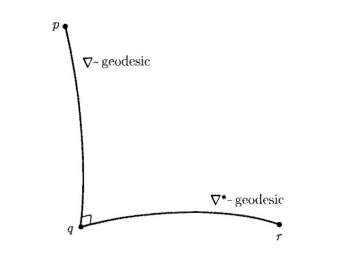
\includegraphics[scale = 0.5]{pythagorean_canonical_divg.png}}
\end{minipage}
\caption{\footnotesize{\textbf{The Pythagorean relation for canonical divergence \citep{amari2007methods}}}}
\label{fig: pythagorean_canonical_divg}
\end{figure}


\item \begin{theorem} (\textbf{Pythagorean Theorem for Canonical Divergence}) \citep{amari2007methods}\\
Let $p$, $q$, and $r$ be three points in $S$ . Let $\gamma_1$ be the \textbf{$\nabla$-geodesic} connecting $p$ and $q$, and let $\gamma_2$ be the  \textbf{$\nabla^{*}$-geodesic} connecting $q$ and $r$. If at the intersection $q$ the curves $\gamma_1$ and $\gamma_2$ are \textbf{orthogonal} (\textbf{with respect to} the inner product $g$), then we have \underline{\textbf{the Pythagorean relation}} (Fig \ref{fig: pythagorean_canonical_divg})
\begin{align}
\divg{}{p}{r} &= \divg{}{p}{q} + \divg{}{q}{r}   \label{eqn: canonical_divg_pythagorean}
\end{align}
\end{theorem}

\begin{figure}
\begin{minipage}[htb]{1\linewidth}
  \centering
  \centerline{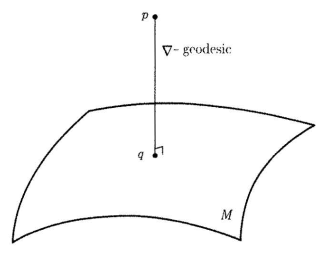
\includegraphics[scale = 0.5]{projection_theorem_canonical_divg.png}}
\end{minipage}
\caption{\footnotesize{\textbf{The Projection theorem for canonical divergence \citep{amari2007methods}}}}
\label{fig: projection_theorem_canonical_divg}
\end{figure}


\item \begin{corollary} (\textbf{Projection Theorem}) \citep{amari2007methods}\\
Let $p$ be a point in $S$ and let $M$ be a submanifold of $S$ which is $\nabla^{*}$-\textbf{autoparallel}. Then a \textbf{necessary and sufficient condition} for a point $q$ in $M$ to satisfy 
\begin{align*}
\divg{}{p}{q} &= \min_{r \in M} \divg{}{p}{r}
\end{align*} is for the \textbf{$\nabla$-geodesic} connecting $p$ and $q$ to be \textbf{orthogonal} to $M$ at $q$.
\end{corollary}

\item \begin{definition}
The point $q$ in the theorem above is called the \underline{\textbf{\emph{$\nabla$-projection of $p$ onto $M$}}}.
\end{definition}

\item \begin{remark}
The \underline{\emph{\textbf{maximum likelihood estimation}}} 
\begin{align*}
\min_{r \in M} \kl{p}{r}
\end{align*} is the \underline{\emph{\textbf{$\nabla^{(m)}$-projection}} or \emph{\textbf{m-projection}} onto $M$}. In other words, the process of maximum likelihood estimation is to \emph{\textbf{match the mean}} of features from the model to the mean of the features from the data.

On the other hand, \underline{\emph{\textbf{the maximum entropy estimation}}}
\begin{align*}
\min_{r \in M} \kl{r}{p}
\end{align*} is the \underline{\emph{\textbf{$\nabla^{(e)}$-projection}} or \emph{\textbf{e-projection}} onto $M$}. In other word, \emph{the process of maximum entropy estimatoin} is to \emph{\textbf{project}} of \emph{the prior distribution} into the \emph{\textbf{exponential family}}.
\end{remark}

\item \begin{theorem}
Let $p$ be a point in $S$ and let $M$ be a submanifold of $S$. A \textbf{necessary and sufficient} condition for a point $q \in M$ to be a \textbf{stationary point}
of the function $\divg{}{p}{\cdot}: r \mapsto  \divg{}{p}{r}$ restricted on $M$ (in other words, the partial derivatives with respect to a coordinate system of $M$ are all $0$) is for the \textbf{$\nabla$-geodesic} connecting $p$ and $q$ to be \textbf{orthogonal} to $M$ at $q$.
\end{theorem}

\item \begin{corollary}
Given a point $p$ in $S$ and a positive number $c$, suppose that the ``D-sphere" $M = \{ q \in S:  \divg{}{p}{q} = c\}$ forms a \textbf{hypersurface} in $S$. Then every
\textbf{$\nabla$-geodesic} passing through the center $p$ \textbf{orthogonally} intersects $M$.
\end{corollary}

\item \begin{remark}
Similarly, \emph{\textbf{\underline{the Hellinger $\alpha$-divergence} in \eqref{eqn: hellinger_alpha_divergence} is a \underline{$(g, \nabla^{(-\alpha)})$-divergence}}}. It is \emph{\textbf{the canonical divergence} with respect to \textbf{dualistic structure}} $(S, g, \nabla^{(-\alpha)}, \nabla^{(\alpha)})$ where $g$ is the Fisher metric.
\end{remark}

\item \begin{remark}
The \emph{\textbf{KL-divergence}} $(\alpha = \pm 1)$ is the \emph{\textbf{only $f$-divergence}} that fits the Pythagorean relation \eqref{eqn: canonical_divg_pythagorean}. The other canonical divergence w.r.t. $(S, g, \nabla^{(-\alpha)}, \nabla^{(\alpha)})$ has similar formula but has an additional product term $\divg{(\alpha)}{p}{q}\divg{(\alpha)}{q}{r}$. 
\end{remark}

%\item \begin{remark} The Bregmen divergence for the negative entropy function 
%\begin{align*}
% \kl{\mb{\mu}_1}{\mb{\mu}_2} &= A^{*}(\mb{\mu}_1) - A^{*}(\mb{\mu}_{2}) - \inn{\mb{\eta}_2}{\mb{\mu}_{1} - \mb{\mu}_{2}}  \\
% &\equiv  A^{*}(\mb{\mu}_1) - A^{*}(\mb{\mu}_{2}) - \inn{\grad{}{A^{*}}(\mb{\mu}_{2})}{\mb{\mu}_{1} - \mb{\mu}_{2}} \nonumber
%\end{align*} is \emph{\textbf{uniquely}} defined on $(S, \nabla^{(e)}, \nabla^{(m)})$ in that it is \emph{\textbf{invariant}} under change of coordinate system.
%\end{remark}
\end{itemize}


\newpage
\bibliographystyle{plainnat}
\bibliography{book_reference.bib}
\end{document}